%\chapter*{Неделя 2}
\protect\thispagestyle{fancy}
\section{}
Гармонический сигнал $x(t) = \cos(2 \pi f_0 t)$, $f_0 = 500$ кГц дискретизован с частотой $f_{d} = 2$ МГц. Изобразить как функцию нормированной частоты $\nu = f/f_{d}$ в диапазоне $|\nu|\leq2$ 
\begin{itemize}
	\item модуль спектра исходного сигнала;
	\item модуль спектра дискретизованного сигнала;
	\item модуль спектра последовательности $z(k) = x(k)\cdot 2\cos(k \pi /2)$.
\end{itemize}


\begin{align*}
	&x(t) = \dfrac{1}{2}e^{j 2 \pi f_d \nu_0 t} + \dfrac{1}{2}e^{-j 2 \pi f_d \nu_0 t},\quad \text{где }\nu_0 = \frac{f_0}{f_d} = \frac{0.5}{2} = \frac{1}{4}.\\
	&z(k) = \dfrac{1}{2}\Big(e^{j 2 \pi \nu_0 k} + e^{-j 2 \pi \nu_0 k}\Big)
	\Big(e^{j \frac{\pi k}{2}} + e^{-j \frac{\pi k}{2}}\Big) =  
	\dfrac{1}{2}\Big(e^{j 2 \pi \frac{1}{2} k} + 2e^{0} + e^{-j 2 \pi \frac{1}{2} k} \Big).
\end{align*}

Спектр исходного и дискретизованного сигналов:\footnote[1]{Часто нормировка весов дельта-функций на $\frac{1}{f_d}$ подразумевается автоматически и может быть опущена.}
\begin{align*}
	&\Capit{X}(f) = \dfrac{1}{2}(\delta(f-f_0)+\delta(f+f_0))
	\quad \Leftrightarrow \quad
	\Capit{X}(\nu) = \dfrac{1}{2f_d}(\delta(\nu-\nu_0) + \delta(\nu+\nu_0)).\\
	&\Capit{X}_d(f) = \dfrac{1}{2}\sum\limits_{m=-\infty}^{+\infty}(\delta(f-f_0-mf_d)+\delta(f+f_0-mf_d)) \quad \Leftrightarrow \quad
	\Capit{X}_d(\nu) = \dfrac{1}{2f_d}\sum\limits_{m=-\infty}^{+\infty}(\delta(\nu-\nu_0-m)+\delta(\nu+\nu_0-m)).
\end{align*}

Спектры последовательности $z(k)$:
\begin{align*}
	&\Capit{Z}(\nu) = \dfrac{1}{2f_d}\Bigg[\delta\Big(\nu+\frac{1}{2}\Big) + 2\delta(\nu) + \delta\Big(\nu-\frac{1}{2}\Big)\Bigg].\\
	&\Capit{Z}_{d}(\nu) = \dfrac{1}{2f_d}\sum\limits_{m=-\infty}^{+\infty}\Bigg[\delta\Big(\nu+\frac{1}{2}-m\Big) +2\delta(\nu-m) + \delta\Big(\nu-\frac{1}{2}-m\Big)\Bigg] =
	\dfrac{1}{f_d}\sum\limits_{m=-\infty}^{+\infty} \Bigg[\delta\Big(\nu-\frac{1}{2}-m\Big) +\delta(\nu-m)\Big)\Bigg].
\end{align*}

\begin{figure}[!h]
	\centering
	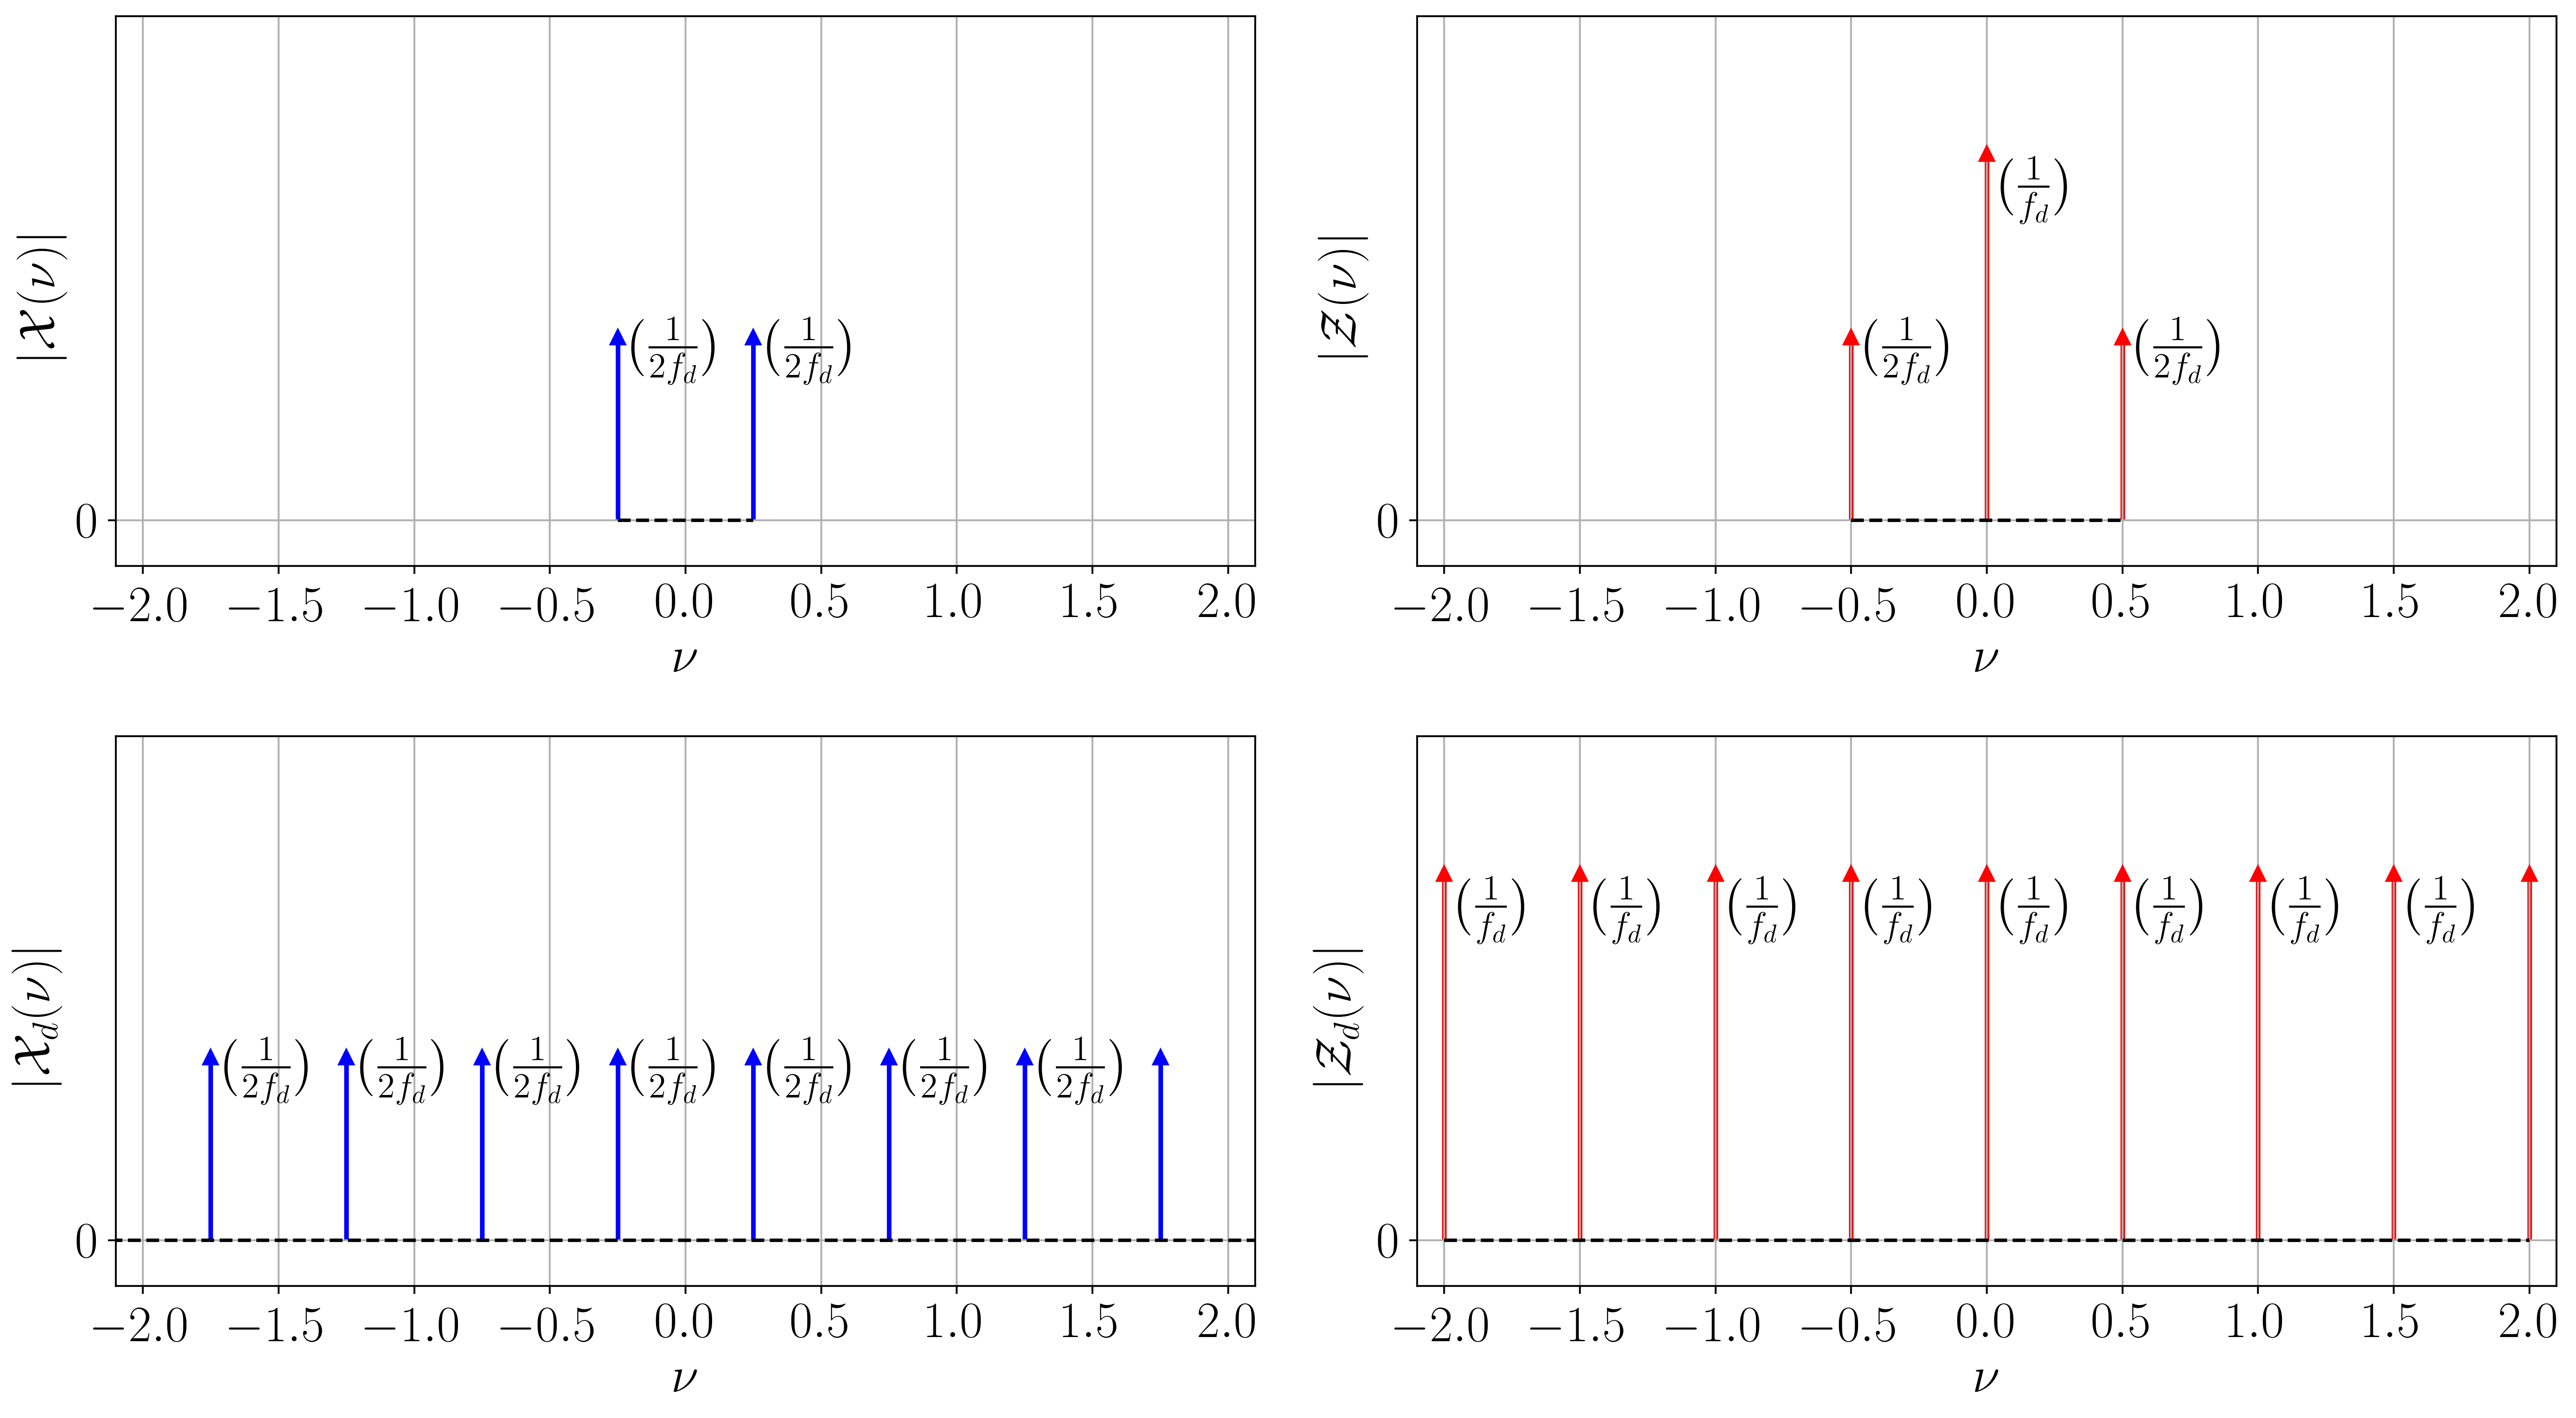
\includegraphics[width=0.90\columnwidth]{pics/fall/2/2-1.png}
	\label{fig:2-1}
\end{figure}


\newpage
\section{}
Сигнал $x(t)$ имеет финитный спектр треугольного вида. Определить коэффициенты ряда Котельникова этого сигнала, полагая, что $\Delta t = \dfrac{1}{2f_{b}}$.

\begin{figure}[!h]
	\centering
	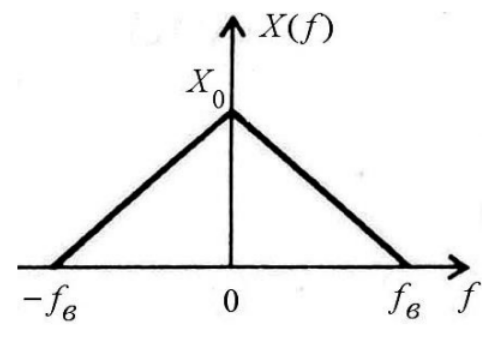
\includegraphics[width=0.20\columnwidth]{pics/fall/2/triangle.png}
	\label{2_triangle}
\end{figure}


\begin{align*}
	c_k &= \dfrac{\braket{x|\phi_k}}{\braket{\phi_k|\phi_k}} = \dfrac{1}{\Delta t} \int\limits_{-\infty}^{+\infty}x(t)\dfrac{\sin(2\pi f_b(t - k \Delta t))}{2\pi f_b(t - k \Delta t)}dt =
	\dfrac{1}{\Delta t} \int\limits_{-\infty}^{+\infty}\Capit{X}(f)\Phi_k(f)df = \int\limits_{-\infty}^{+\infty}\Capit{X}(f) e^{j 2\pi f k \Delta t} \Theta \big(-f_b \leq  f \leq f_{b}\big) df =\\
	&=\int\limits_{-f_b}^{+f_b}\Capit{X}(f) e^{j 2\pi f k \Delta t}df = \dfrac{\Capit{X}_0}{f_b}\Bigg\{\int\limits_{-f_b}^{0} (f_b + f) e^{j 2\pi f k \Delta t}df + \int\limits_{0}^{f_b} (f_b - f) e^{j 2\pi f k \Delta t}df\Bigg\} =\\
	&=\dfrac{\Capit{X}_0}{j2\pi k f_b \Delta t}\Bigg\{(f_b + f)e^{j 2\pi f k \Delta t}\Bigg|_{-f_b}^0 + (f_b - f)e^{j 2\pi f k \Delta t}\Bigg|_{0}^{f_b}
	- \int\limits_{-f_b}^{0} e^{j 2\pi f k \Delta t}df + \int\limits_{0}^{f_b} e^{j 2\pi f k \Delta t}df\Bigg\} = \\
	&=\dfrac{\Capit{X}_0}{j\pi k}\Bigg\{f_b - f_b + \dfrac{1}{j 2\pi k \Delta t} \Bigg(e^{j 2\pi f k \Delta t}\Bigg|_{0}^{f_b} - e^{j 2\pi f k \Delta t}\Bigg|_{-f_b}^{0} \Bigg) \Bigg\} =
	\dfrac{\Capit{X}_0}{(j\pi k)^2 2\Delta t}\Bigg\{-2 + e^{j 2\pi f_b k \Delta t} + e^{-j 2\pi f_b k \Delta t} \Bigg \} = \\
	&= \dfrac{\Capit{X}_0}{(\pi k)^2 \Delta t} - \dfrac{\Capit{X}_0}{(\pi k)^2 \Delta t}\cos(2\pi f_b k \Delta t) = \dfrac{\Capit{X}_0}{(\pi k)^2 \Delta t} - \dfrac{\Capit{X}_0}{(\pi k)^2 \Delta t}\cos(\pi k) = \dfrac{2\Capit{X}_0}{(\pi k)^2 \Delta t}\sin^2 \Big(\frac{\pi k}{2}\Big) = \dfrac{4 \Capit{X}_0 f_b}{(\pi k)^2}\sin^2 \Big(\frac{\pi k}{2}\Big).
\end{align*}

\section{}
Найти и изобразить по модулю ДВПФ $16$-точечных последовательностей:
\begin{equation*}
	x(k) = \sum \limits_{m=0}^{15}\mathbf{1}(k-m) \quad \text{и}\quad y(k) = x(k)z(k),\text{ где }z(k) = \cos\Big(2 \pi k \frac{3}{16}\Big).
\end{equation*}

\begin{align*}
	&\Capit{X}_{N}(\nu) = \sum \limits_{k = 0}^{N-1} x(k)e^{-j2\pi \nu k} = \sum \limits_{k = 0}^{N-1} e^{-j2\pi \nu k} = 
	\dfrac{1 - e^{-j 2 \pi \nu N}}{1 - e^{-j 2 \pi \nu}} = \dfrac{e^{-j \pi \nu N}}{e^{-j \pi \nu}} 
	\dfrac{e^{j \pi \nu N} - e^{-j \pi \nu N}}{e^{j \pi \nu} - e^{-j \pi \nu}} = e^{-j \pi \nu (N-1)}\dfrac{\sin(N \pi \nu)}{\sin(\pi \nu)}.\\
	&\Capit{Z}(\nu) = \sum \limits_{k = -\infty}^{+\infty} z(k)e^{-j2\pi \nu k} = \dfrac{1}{2}\sum \limits_{k=-\infty}^{+\infty} e^{-j2\pi \big(\nu - \frac{3}{16}\big) k} + \dfrac{1}{2}\sum \limits_{k =-\infty}^{+\infty} e^{-j2\pi \big(\nu + \frac{3}{16}\big) k} = \dfrac{1}{2}\sum \limits_{m = -\infty}^{+\infty}\Big[\delta\big(\nu - \frac{3}{16}-m\big) + \delta\big(\nu + \frac{3}{16}-m\big)\Big].\\
	&\Capit{Y}(\nu) = \int \limits_{-\frac{1}{2}}^{\frac{1}{2}}\Capit{X}_{16}(\tilde{\nu})\Capit{Z}(\nu - \tilde{\nu})d\tilde{\nu} = \dfrac{1}{2}\int \limits_{-\frac{1}{2}}^{\frac{1}{2}}\Capit{X}_{16}(\tilde{\nu})\sum \limits_{m = -\infty}^{+\infty}\Big[\delta\big(\nu - \tilde{\nu} - \frac{3}{16}-m\big) + \delta\big(\nu - \tilde{\nu} + \frac{3}{16}-m\big)\Big]d \tilde{\nu} =\\
	&=\dfrac{1}{2}\Capit{X}_{16} \big(\nu - \frac{3}{16}\big) + \dfrac{1}{2}\Capit{X}_{16} \big(\nu + \frac{3}{16}\big) = e^{-j \pi 15(\nu - \frac{3}{16})}\dfrac{\sin(16 \pi (\nu - \frac{3}{16}))}{2\sin(\pi (\nu - \frac{3}{16}))} + 
	e^{-j \pi 15(\nu + \frac{3}{16})}\dfrac{\sin(16 \pi (\nu + \frac{3}{16}))}{2\sin(\pi (\nu + \frac{3}{16}))}.
\end{align*}


\begin{figure}[!h]
	\centering
	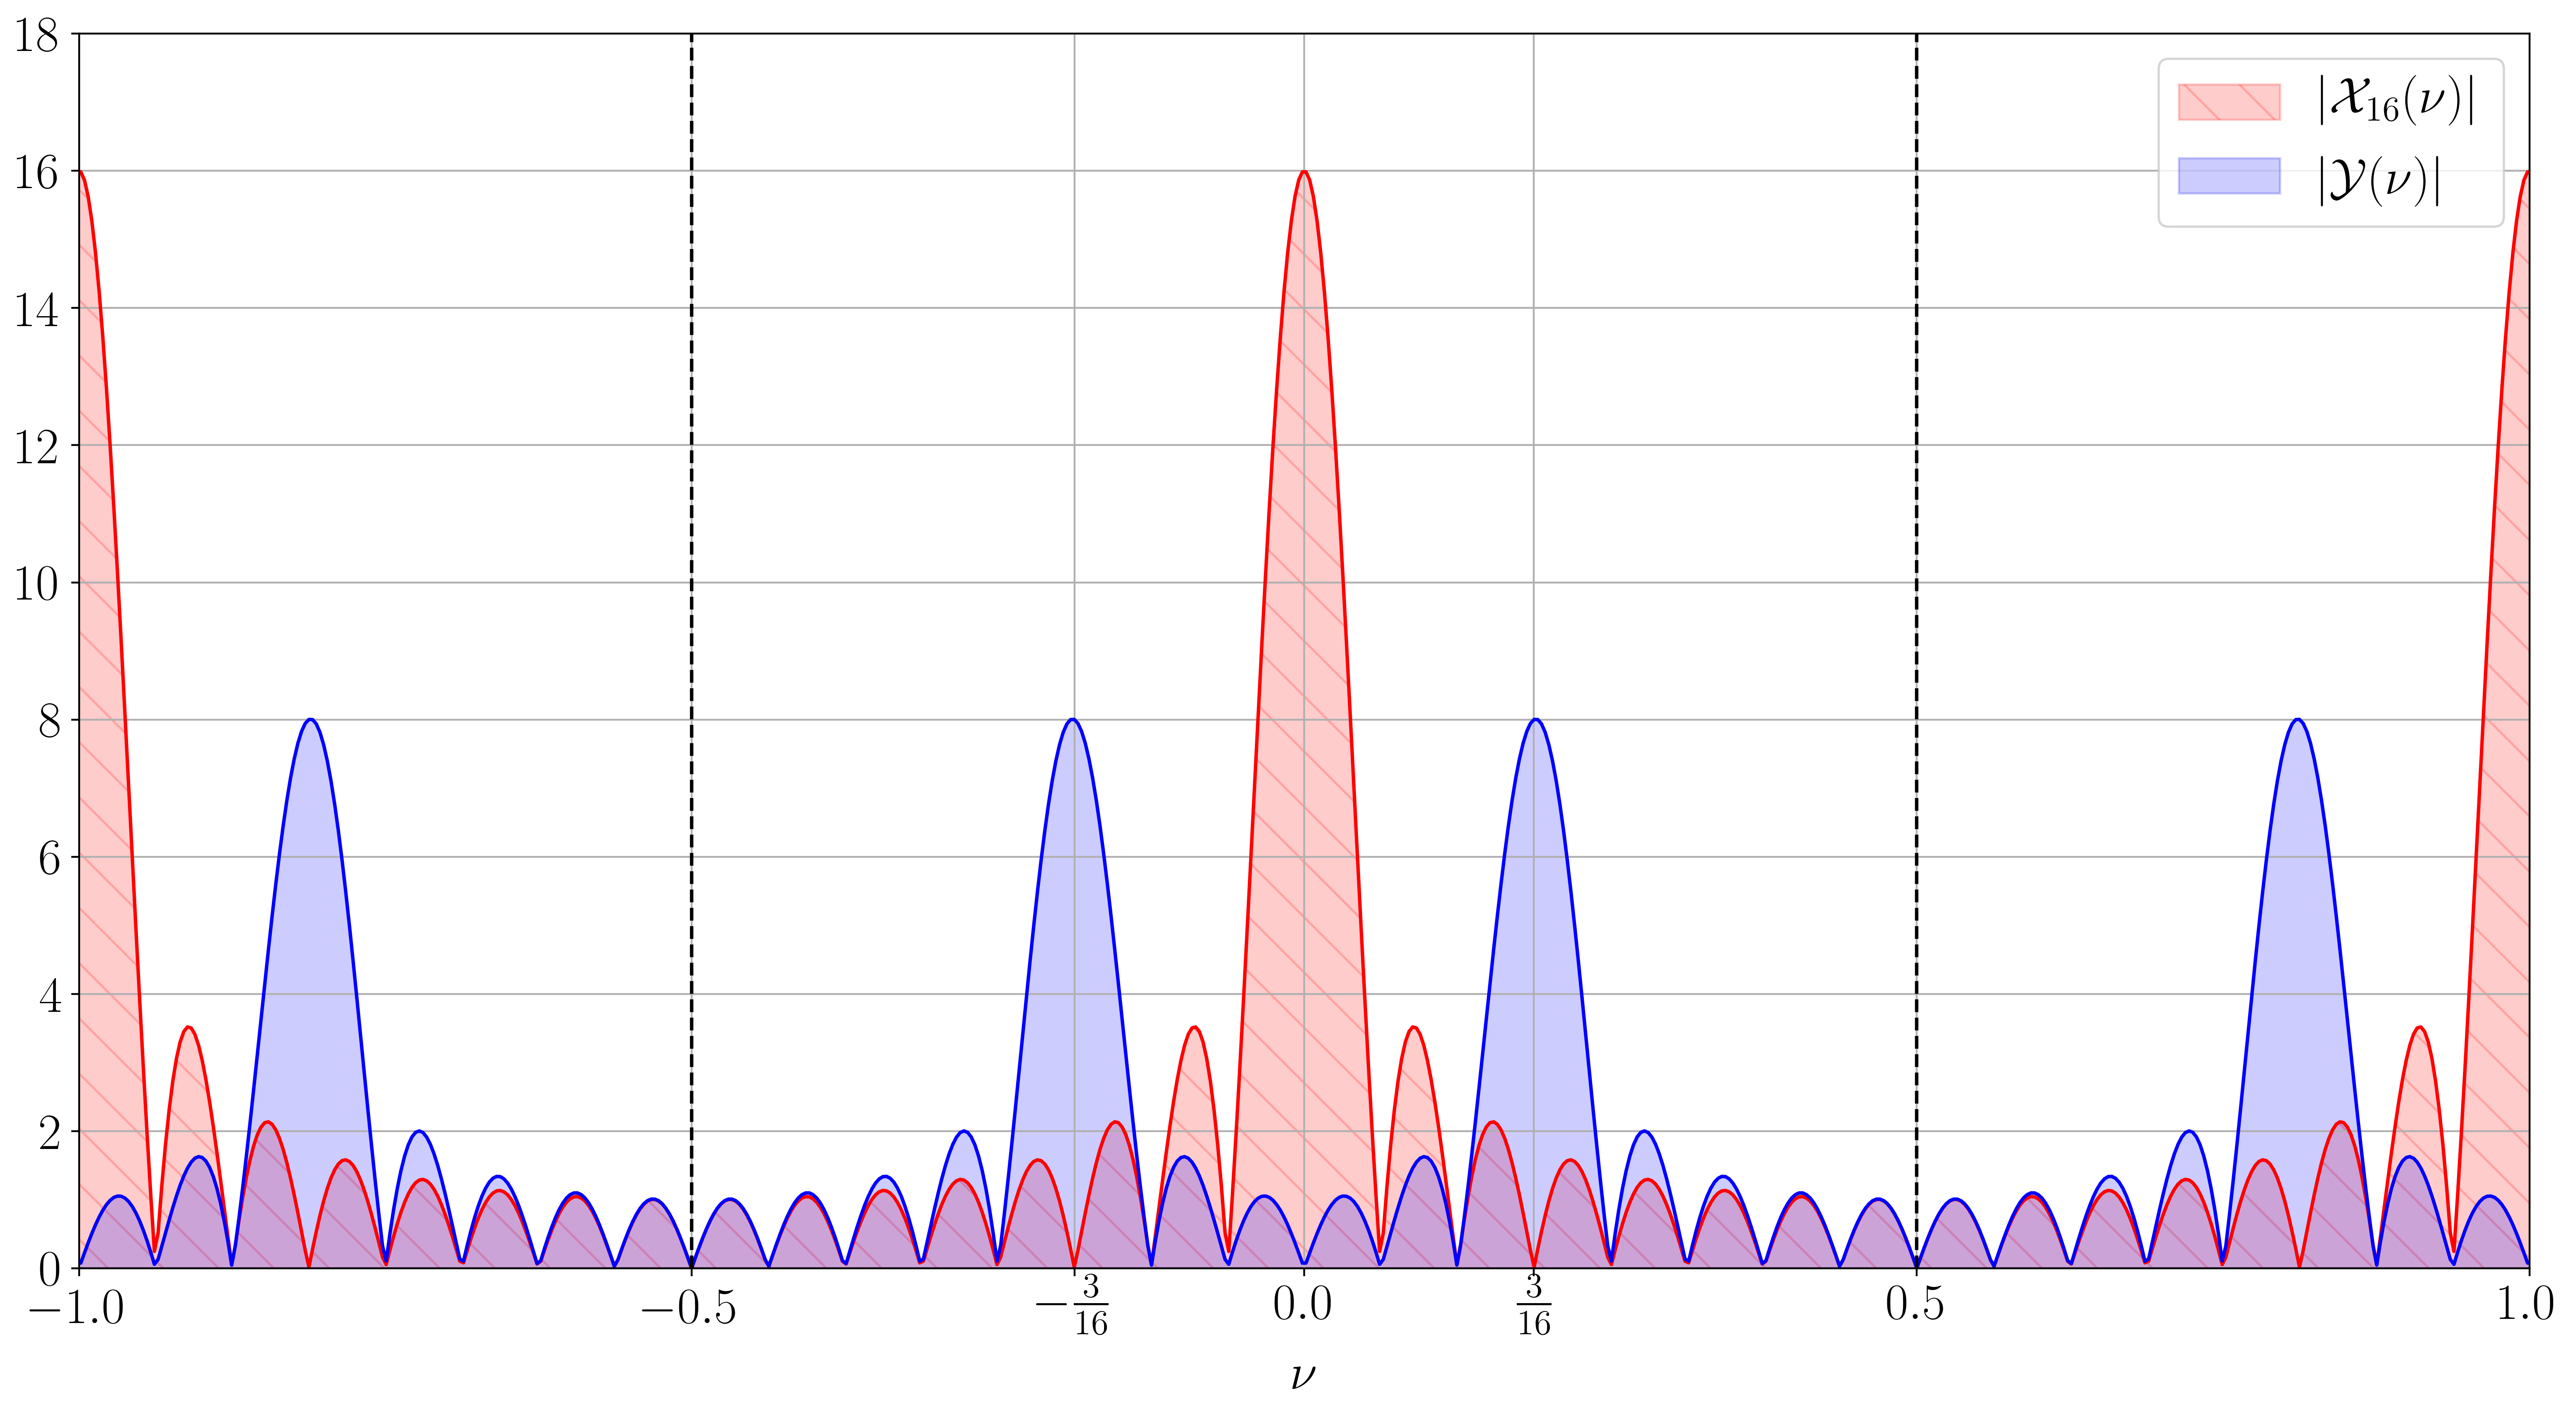
\includegraphics[width=1.0\columnwidth]{pics/fall/2/2-3.png}
	\label{fig:2-3}
\end{figure}


\section{}
Сформулировать и доказать теорему о свёртке последовательностей для ДВПФ.

\textit{Теорема:}

Пусть $\Capit{X}(\nu) = \sum\limits_{k = -\infty}^{+\infty}x(k)e^{-j 2 \pi \nu k}$ и $\Capit{Y}(\nu) = \sum\limits_{k = -\infty}^{+\infty}y(k)e^{-j 2 \pi \nu k}$, тогда дискретной свёртке двух сигналов $z(k) = \sum \limits_{m = -\infty}^{+\infty} x(m)y(k-m)$ отвечает произведение их спектров $\Capit{Z}(\nu) = \Capit{X}(\nu)\Capit{Y}(\nu)$.

\textit{Доказательство:}
\begin{align*}
	\Capit{Z}(\nu) &= \sum\limits_{k = -\infty}^{+\infty}z(k)e^{-j 2 \pi \nu k} = \sum\limits_{k = -\infty}^{+\infty} \sum\limits_{m = -\infty}^{+\infty} x(m)y(k-m) e^{-j 2 \pi \nu m} e^{-j 2 \pi \nu (k - m)}  = \\
	&= \sum\limits_{m = -\infty}^{+\infty} x(m) e^{-j 2 \pi \nu m} \sum\limits_{n = -\infty}^{+\infty} y(n) e^{-j 2 \pi \nu n} = \sum\limits_{m = -\infty}^{+\infty} x(m) e^{-j 2 \pi \nu m} \Capit{Y}(\nu) = \Capit{X}(\nu) \Capit{Y}(\nu).
\end{align*}
